\documentclass[10pt]{article}
 
\usepackage[margin=1.5cm]{geometry} 
\usepackage{amsmath,amsthm,amssymb}
\usepackage{polski}
\usepackage[utf8]{inputenc}
\usepackage{siunitx}
\usepackage{graphicx}
\usepackage{comment}


 
\newenvironment{theorem}[2][Twierdzenie]{\begin{trivlist}
\item[\hskip \labelsep {\bfseries #1}\hskip \labelsep {\bfseries #2.}]}{\end{trivlist}}
\newenvironment{question}[2][Pytanie]{\begin{trivlist}
\item[\hskip \labelsep {\bfseries #1}\hskip \labelsep {\bfseries #2.}]}{\end{trivlist}}
\newenvironment{hypothesis}[2][Hipoteza]{\begin{trivlist}
\item[\hskip \labelsep {\bfseries #1}\hskip \labelsep {\bfseries #2.}]}{\end{trivlist}}
\newenvironment{lemma}[2][Lemat]{\begin{trivlist}
\item[\hskip \labelsep {\bfseries #1}\hskip \labelsep {\bfseries #2.}]}{\end{trivlist}}
\newenvironment{exercise}[2][Ćwiczenie]{\begin{trivlist}
\item[\hskip \labelsep {\bfseries #1}\hskip \labelsep {\bfseries #2.}]}{\end{trivlist}}
\newenvironment{reflection}[2][Uwaga]{\begin{trivlist}
\item[\hskip \labelsep {\bfseries #1}\hskip \labelsep {\bfseries #2.}]}{\end{trivlist}}
\newenvironment{proposition}[2][Założenie]{\begin{trivlist}
\item[\hskip \labelsep {\bfseries #1}\hskip \labelsep {\bfseries #2.}]}{\end{trivlist}}
\newenvironment{corollary}[2][Wniosek]{\begin{trivlist}
\item[\hskip \labelsep {\bfseries #1}\hskip \labelsep {\bfseries #2.}]}{\end{trivlist}}
 
\begin{document}

\title{Implementacja algorytmu eliminacji Gaussa\\oraz testy wydajnościowe i obliczeniowe trzech określonych typów}
\author{Grams, Stanisław\\Jezierski, Maciej\\Korczakowski, Juliusz\\ MFI UG\\Algorytmy Numeryczne}

\maketitle
\section {Operacje na macierzach}
\subsection{O sprawozdaniu}
Sprawozdanie prezentuje analizę wydajności i poprawności implementacji algorytmu eliminacji Gaussa, dla macierzy kwadratowej $A$ oraz wektora $B$ w układzie liniowym $A*X = B$ gdzie współczynniki wektora $A$ oraz macierzy kwadratowej $X$ są losowane. \\
Zakres losowanych współczynników jest równy $[-1, 1]$, natomiast każdy z nich został wyznaczony według wzoru $r/2^{16}$, gdzie $r$ jest losową liczbą całkowitą z zakresu $[-2^{16} , 2^{16}]$.
Wygenerowany w ten sposób wektor $X$ pozostaje próbą kontrolną natomiast do algorytmu jako parametr przekazujemy wyliczony według powyższego wzoru wektor $B$.
\subsection{O implementacji}
Program \textit{„gauss”} został napisany w języku C++ z użyciem bibliotek:
\begin{itemize}
    \item \textit{„gmp.h”} — pozwalającej zaimplementować wymagany typ całkowity (TC)
    \item \textit{„pthread.h”} — do celów obsługi wielowątkowości,
\end{itemize}
Wyniki działania programu zapisywane są do poszczególnych plików \textit{*.csv}.
Zaimplementowano następujące warianty algorytmu Gaussa dla kolejnych typów zmiennych rzeczywistych:
\begin{itemize}
\item[] Warianty algorytmu eliminacji
    \item G: bez wyboru elementu podstawowego,
    \item PG: z częściowym wyborem elementu podstawowego, 
    \item FG: z całkowitym wyborem elementu podstawowego.
\item[] Typy zmiennych rzeczywistych
    \item {float} – wbudowany typ pojedynczej precyzji 
    \item {double} – wbudowany typ podwójnej precyzji
    \item {MyType} – typ zaimplementowany przez zespół, oparty o bibliotekę „GMP.h” i typ „mpq\_t”
\end{itemize}

\section {Poprawność hipotez}
\subsection{Czas wykonywania}
\begin{hypothesis}{1}
Dla dowolnego ustalonego rozmiaru macierzy czas działania metody Gaussa w kolejnych wersjach (G,PG,FG) rośnie.
\end{hypothesis}
Analiza wykresów przedstawiających dla typów float oraz double (typ własny pomijamy na rzecz trzeciej hipotezy), pozwala na wyciągnięcie następujących wniosków:\\
1. W przypadku typów float oraz double kolejne typy metody Gaussa wykazują coraz większą czasochłonność jednak największą różnicę widać pomiędzy FG a pozostawłymi.\\
2. W przypadku typu własnego różnice są minimalne, mimo tendencji potwierdzającej hipotezę zdarzają się momenty w których wykres jej przeczy.\\
3. W przypadku typu własnego wzrost jest prawie paraboliczy, jednak dla typów float oraz double krzywe wykresów są z początku bardzo nieregularne aby potem zbliżyć się do paraboli.\\
\begin{corollary}{1}
Hipoteza potwierdza się w pełni dla typów float oraz double, typ własny w większej części wykresu zdaje się jej nie przeczyć, jednak niektórych momentach wykres układa się wbrew hipotezie.
\end{corollary}

\begin{figure}[!htb]
   \begin{minipage}{0.48\textwidth}
     \centering
     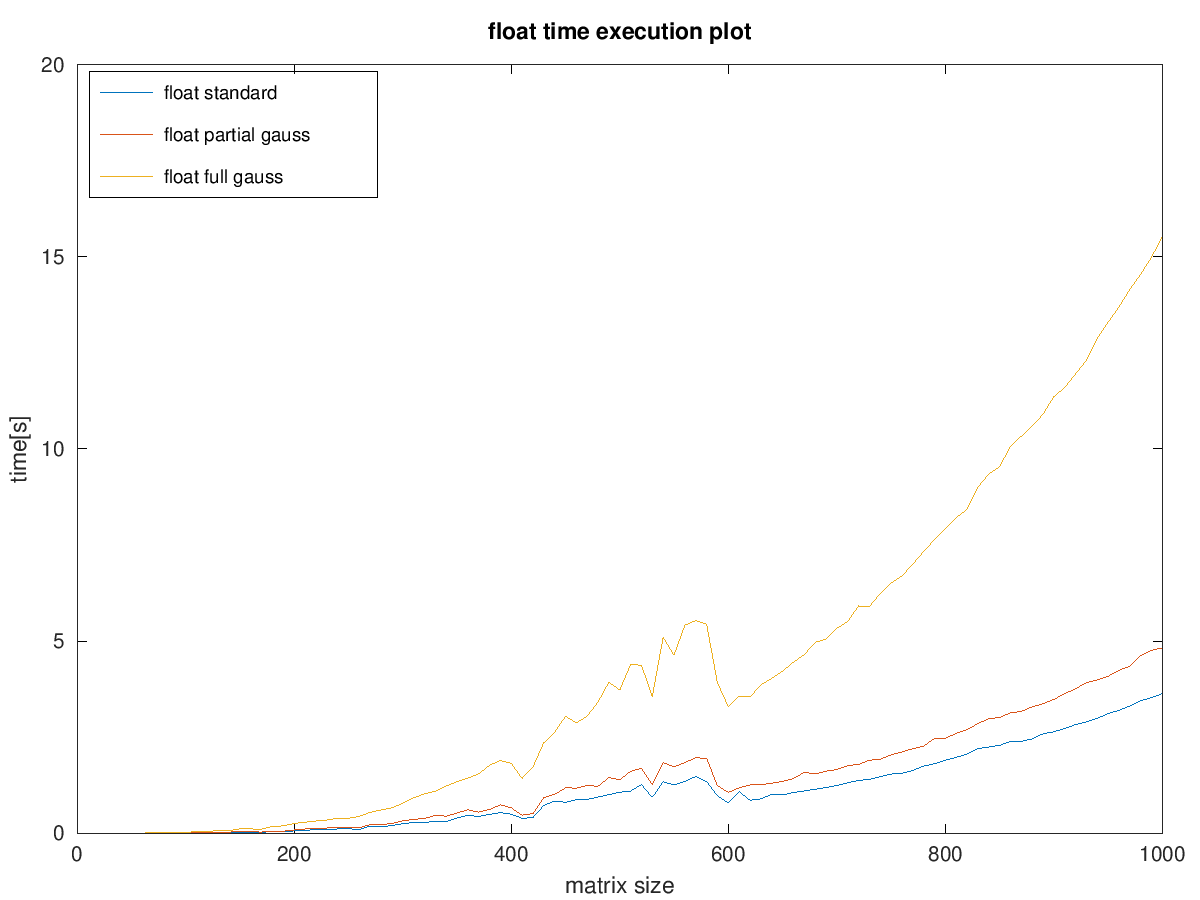
\includegraphics[width=.7\linewidth]{00_float_plot_time}
     \caption{Czas dla float}\label{Fig:Data1}
   \end{minipage}\hfill
   \begin{minipage}{0.48\textwidth}
     \centering
     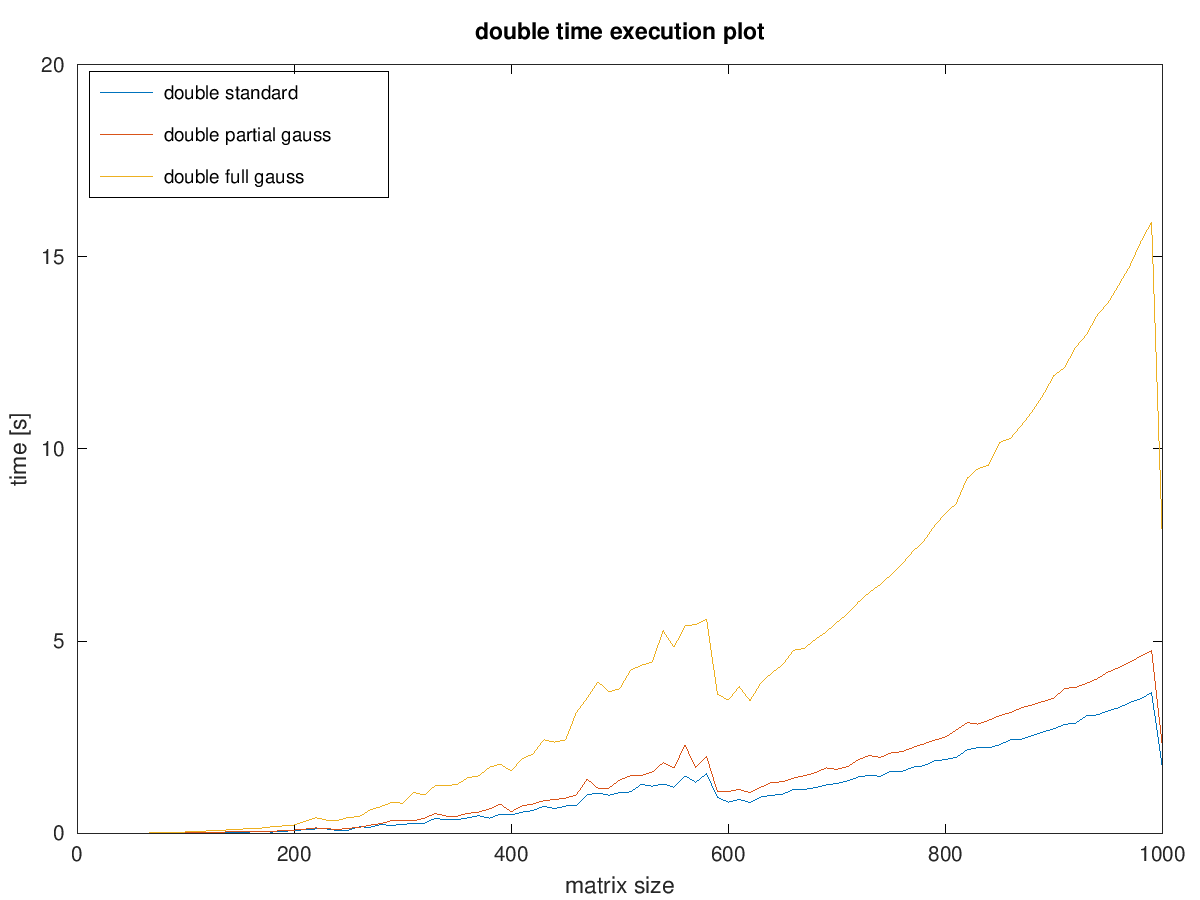
\includegraphics[width=.7\linewidth]{01_double_plot_time}
     \caption{Czas dla double}\label{Fig:Data2}
   \end{minipage}
\end{figure}
\begin{figure}[!htb]
\centering
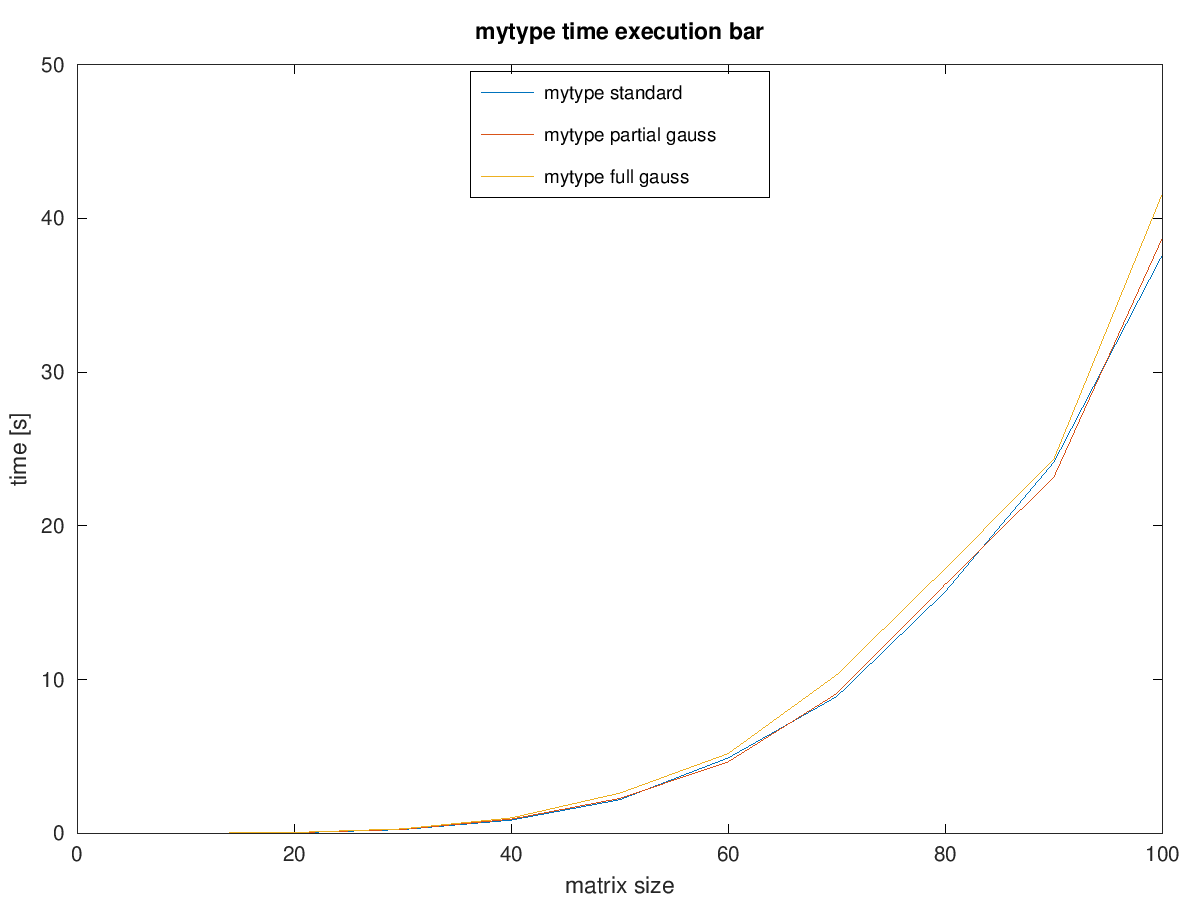
\includegraphics[width=.7\linewidth]{02_mytype_plot_time.png}\\
\caption{Czas dla typu własnego}
\end{figure}


\subsection{Błąd wyniku}
\begin{hypothesis}{2}
Dla dowolnego ustalonego rozmiaru macierzy błąd uzyskanego wyniku metody Gaussa w kolejnych wersjach (G, PG, FG) maleje.\end{hypothesis}
Analiza wykresów przedstawiających błędy obliczeń dla typów float oraz double (typ własny pomijamy na rzecz trzeciej hipotezy), pozwala na wyciągnięcie następujących wniosków: \\
1. Kolejne typy metody Gaussa zmniejszają błędy zarówno względne jak i bezwzględne.\\
2. Względem standardowej, metody PG i FG mają wyraźnie większą dokładność.\\
3. Dokładność metody FG jest zdecydowanie najwyższa oraz bliska pełnej.\\
4. Typ float wykazuje znacznie mniejszą dokładność (kilka rzędów wielkości) od double co jest spowodowane różnicą w precyzjy obu typów.\\
\begin{corollary}{2}
Hipoteza jest prawdziwa - kolejne typy metody Gaussa zwiększają dokładność wyników, największą róznicę widać między metodą standardową a pozostałymi.
\end{corollary}

\begin{figure}[!htb]
   \begin{minipage}{0.48\textwidth}
     \centering
     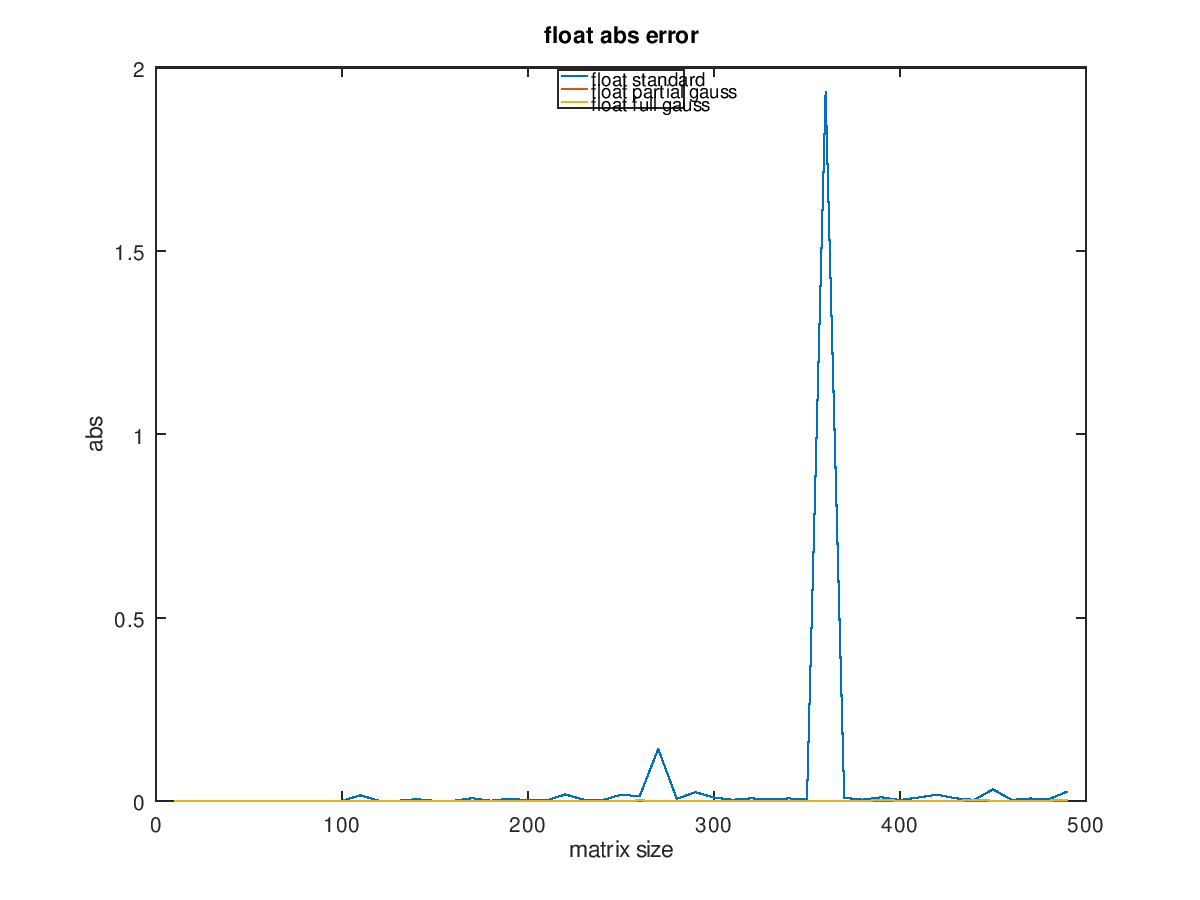
\includegraphics[width=.7\linewidth]{03_float_plot_abs}
     \caption{Błąd absolutny dla float}\label{Fig:Data1}
   \end{minipage}\hfill
   \begin{minipage}{0.48\textwidth}
     \centering
     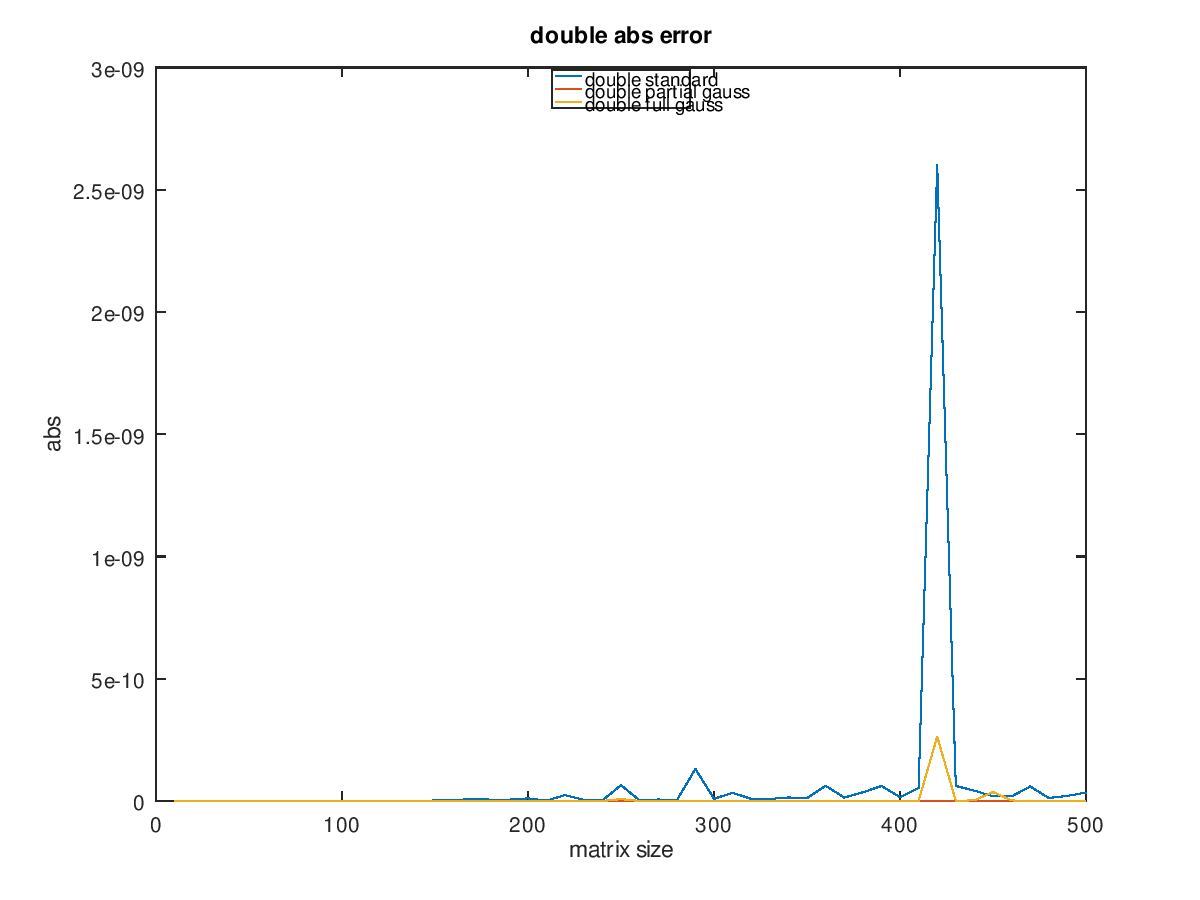
\includegraphics[width=.7\linewidth]{04_double_plot_abs}
     \caption{Błąd absolutny dla double}\label{Fig:Data2}
   \end{minipage}
\end{figure}
\begin{figure}[!htb]
   \begin{minipage}{0.48\textwidth}
     \centering
     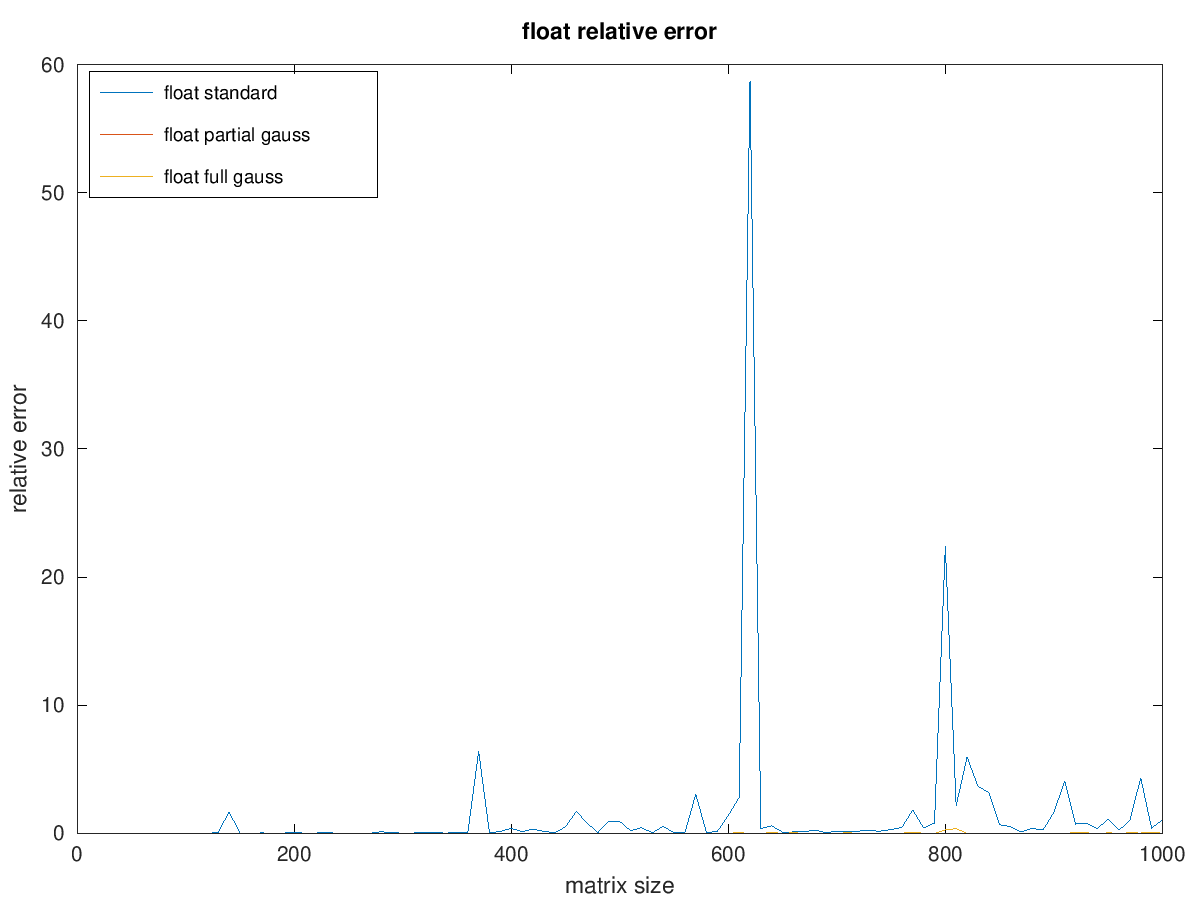
\includegraphics[width=.7\linewidth]{05_float_plot_rel}
     \caption{Błąd względny dla float}\label{Fig:Data1}
   \end{minipage}\hfill
   \begin{minipage}{0.48\textwidth}
     \centering
     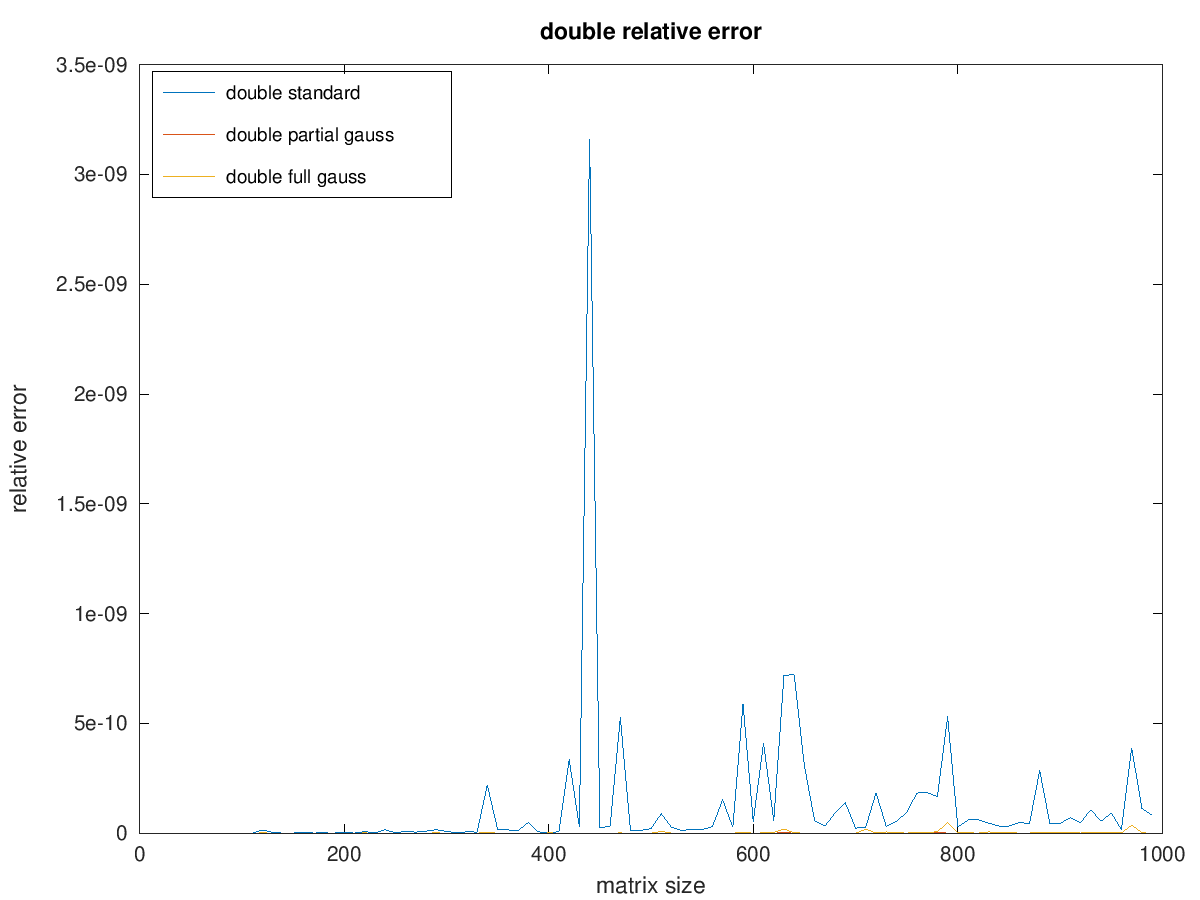
\includegraphics[width=.7\linewidth]{06_double_plot_rel}
     \caption{Błąd względny dla double}\label{Fig:Data2}
   \end{minipage}
\end{figure}

\subsection{Bezbłędność własnej arytmetyki na ułamkach}
\begin{hypothesis}{3}
Użycie własnej arytmetyki na ułamkach zapewnia bezbłędne wyniki niezależnie od wariantu metody Gaussa i rozmiaru macierzy.
\end{hypothesis}
Z analizy tabeli (Tabela 1) wynika, że wszystkie błędy obliczeń wykonywanych na własnym typie ułamkowym są równe zeru. Z powyższej obserwacji można wyciągnąć wniosek, że własna artmetyka ułamków przechowująca licznik oraz mianownik skutecznie eliminuje błąd obliczeń. Warto jednak zaznaczyć, że powyższą skuteczość własny typ ułamkowy zawdzięcza typowi zmiennej, w której jest przechowywany licznik oraz mianownik. Nasz typ oparliśmy o bibliotekę GMP, co daje praktycznie pełną dokładność nawet dla skomplikowanych obliczeń na liczbach wymiernych.
\begin{corollary}{3}
Hipoteza jest prawdziwa - poprawnie zaimplementowany typ ułamkowy daje pełną dokładność.
\end{corollary}

\begin{figure}[!htb]
\centering
\includegraphics[width=.7\linewidth]{tabela.png}\\
\caption{Czasy oraz błędy dla typu własnego}\label{Fig:Data2}
\end{figure}


\section {Odpowiedzi na zadane pytania}
\begin{question}{1}
Jak zależy dokładność obliczeń (błąd) od rozmiaru macierzy dla dwóch wybranych przez Ciebie wariantów metody Gaussa gdy obliczenia prowadzone są na typie podwójnej precyzji (TD)?
\end{question}
W przypadku anlizowania metody standardowej dla obu wbudowanych typów ułamkowych można zauważyć pewną prawidłowość, dla mniejszych macierzy błędy są znikome, jednak począwszy od wielkości nieco mniejszych niż 400 błędy stają się większe, natomiast po powiększeniu wielkości macierzy pozostają na podobnym poziomie.

\begin{question}{2}
Jak przy wybranym przez Ciebie wariancie metody Gaussa zależy czas działania algorytmu od rozmiaru macierzy i różnych typów?
\end{question}
Analizuje danych dla metody FG.\\
W przypadku typu własnego wzrost jest prawie paraboliczy, jednak dla typów wbudowanych do wielkości macierzy rzędu 600 krzywa obrazująca wzrost czasu jest bardzo nieregularna aby po przekroczeniu tej wielkości być zbliżoną do paraboli. 

\section {Wydajność implementacji}
\begin{exercise}{2}
Podaj czasy rozwiązania układu równań uzyskane dla macierzy o rozmiarze 500 dla 9 testowanych wariantów.
\end{exercise}
W naszym przypadku czas wykonania algorytmu dla macierzy o wielkości 500x500 prezentuje się następująco (czas dla typu własnego został wyliczony w przybliżeniu według danych uzyskanych w wyniku działania programu):\\
\begin{center}
\begin{figure}[!htb]
\centering
\includegraphics[width=.7\linewidth]{czasywykonania.png}\\
\caption{Czasy wykonania dla macierzy 500x500}\label{Fig:Data2}
\end{figure}
\end{center}
\vspace{-1.5cm}
\section {Podział pracy nad projektem}
\vspace{-0.5cm}
\begin{figure}[!htb]
\centering
\includegraphics[scale=0.3]{podzial.png}
\end{figure}
\end{document}
